\subsubsection{Versuch: Nachweis der hohen Lichtdurchlässigkeit von PC und der einfachen Weiterverarbeitung}

Material:
\begin{itemize*}
    \item handelsübliche CD, Schere, 2 Glasschalen, Plätzchenform, Pinzette, Alufolie, Heizplatte
    \item Chemikalien: Salpetersäure (Sicherheitshinweis: CAS Nr. 7697-37-2 (\autoref{fig:cdbrandfoerdernd}, \autoref{fig:cdaetzwirkung}))
\end{itemize*}

\begin{figure}[h]
    \begin{center}
        \begin{minipage}[t]{0.4\textwidth}
            \begin{center}
                \includegraphics[height=0.1\textheight]{Bilder/Optische_Datentraeger_Die_Compact_Disc/Material_Polycarbonat/cdbrandfoerdernd.png}
                \caption[brandfördernder Stoff \newline \url{https://upload.wikimedia.org/wikipedia/commons/e/e5/GHS-pictogram-rondflam.svg} (zuletzt aufgerufen am 19.09.2015)]{brandfördernder Stoff}
                \label{fig:cdbrandfoerdernd}
            \end{center}
        \end{minipage}
        \hspace{0.025\textwidth}
        \begin{minipage}[t]{0.4\textwidth}
            \begin{center}
                \includegraphics[height=0.1\textheight]{Bilder/Optische_Datentraeger_Die_Compact_Disc/Material_Polycarbonat/cdaetzwirkung.png}
                \caption[ätzender Stoff \newline \url{https://upload.wikimedia.org/wikipedia/commons/a/a1/GHS-pictogram-acid.svg} (zuletzt aufgerufen am 19.09.2015)]{ätzender Stoff}
                \label{fig:cdaetzwirkung}
            \end{center}
        \end{minipage}
    \end{center}
\end{figure}

Schutzvorkehrungen:
\begin{itemize}
    \item Abzug, Schutzkleidung, Handschuhe, Schutzbrille
\end{itemize}

Versuchsablauf:
\begin{enumerate*}
    \item Die CD wird in eine der Glasschalen gelegt und mit Salpetersäure übergossen (siehe \autoref{fig:cdsalpeter}). Dies muss unter einem Abzug geschehen, da nitrose Gase entstehen.
    \item Nach kurzer Zeit \glqq quellen\grqq{} die Lack- und die Aluminiumschicht auf (siehe \autoref{fig:cdquillt}) und lassen sich mithilfe der Pinzette entfernen.
    \item Die \glqq gehäutete\grqq{} CD wird nun in die zweite Glasschale gelegt und vorsichtig unter dem Wasserhahn abgespült. \autoref{fig:cdblank} zeigt die resultierende Polycarbonatscheibe\footnote{Zu diesem Zeitpunkt kann die hohe Lichtdurchlässigkeit der Polycarbonatscheibe überprüft werden.}.
    \item Die Polycarbonatscheibe wird nun in kleine Stücke zerschnitten, die nicht größer als 1 cm² sind (siehe \autoref{fig:cdzerschnitten}).
    \item Die Polycarbonatschnipsel werden ca. 1 cm hoch in die Plätzchenform gefüllt, welche sich auf der mit Aluminiumfolie bedeckten Heizplatte befindet (siehe \autoref{fig:cdschmelzen}).
    \item Die Heizplatte wird auf über 250°C erhitzt und man wartet bis das Polycarbonat zu einer gleichmäßigen Oberfläche zerflossen ist.
    \item Die Heizplatte wird nun ausgeschalten. Nach dem Abkühlen kann das \glqq Polycarbonatplätzchen\grqq{} aus der Form gebrochen werden (siehe \autoref{fig:cdplaetzchen}).
\end{enumerate*}

\begin{figure}[h]
    \begin{center}
        \begin{minipage}[t]{0.4\textwidth}
            \begin{center}
                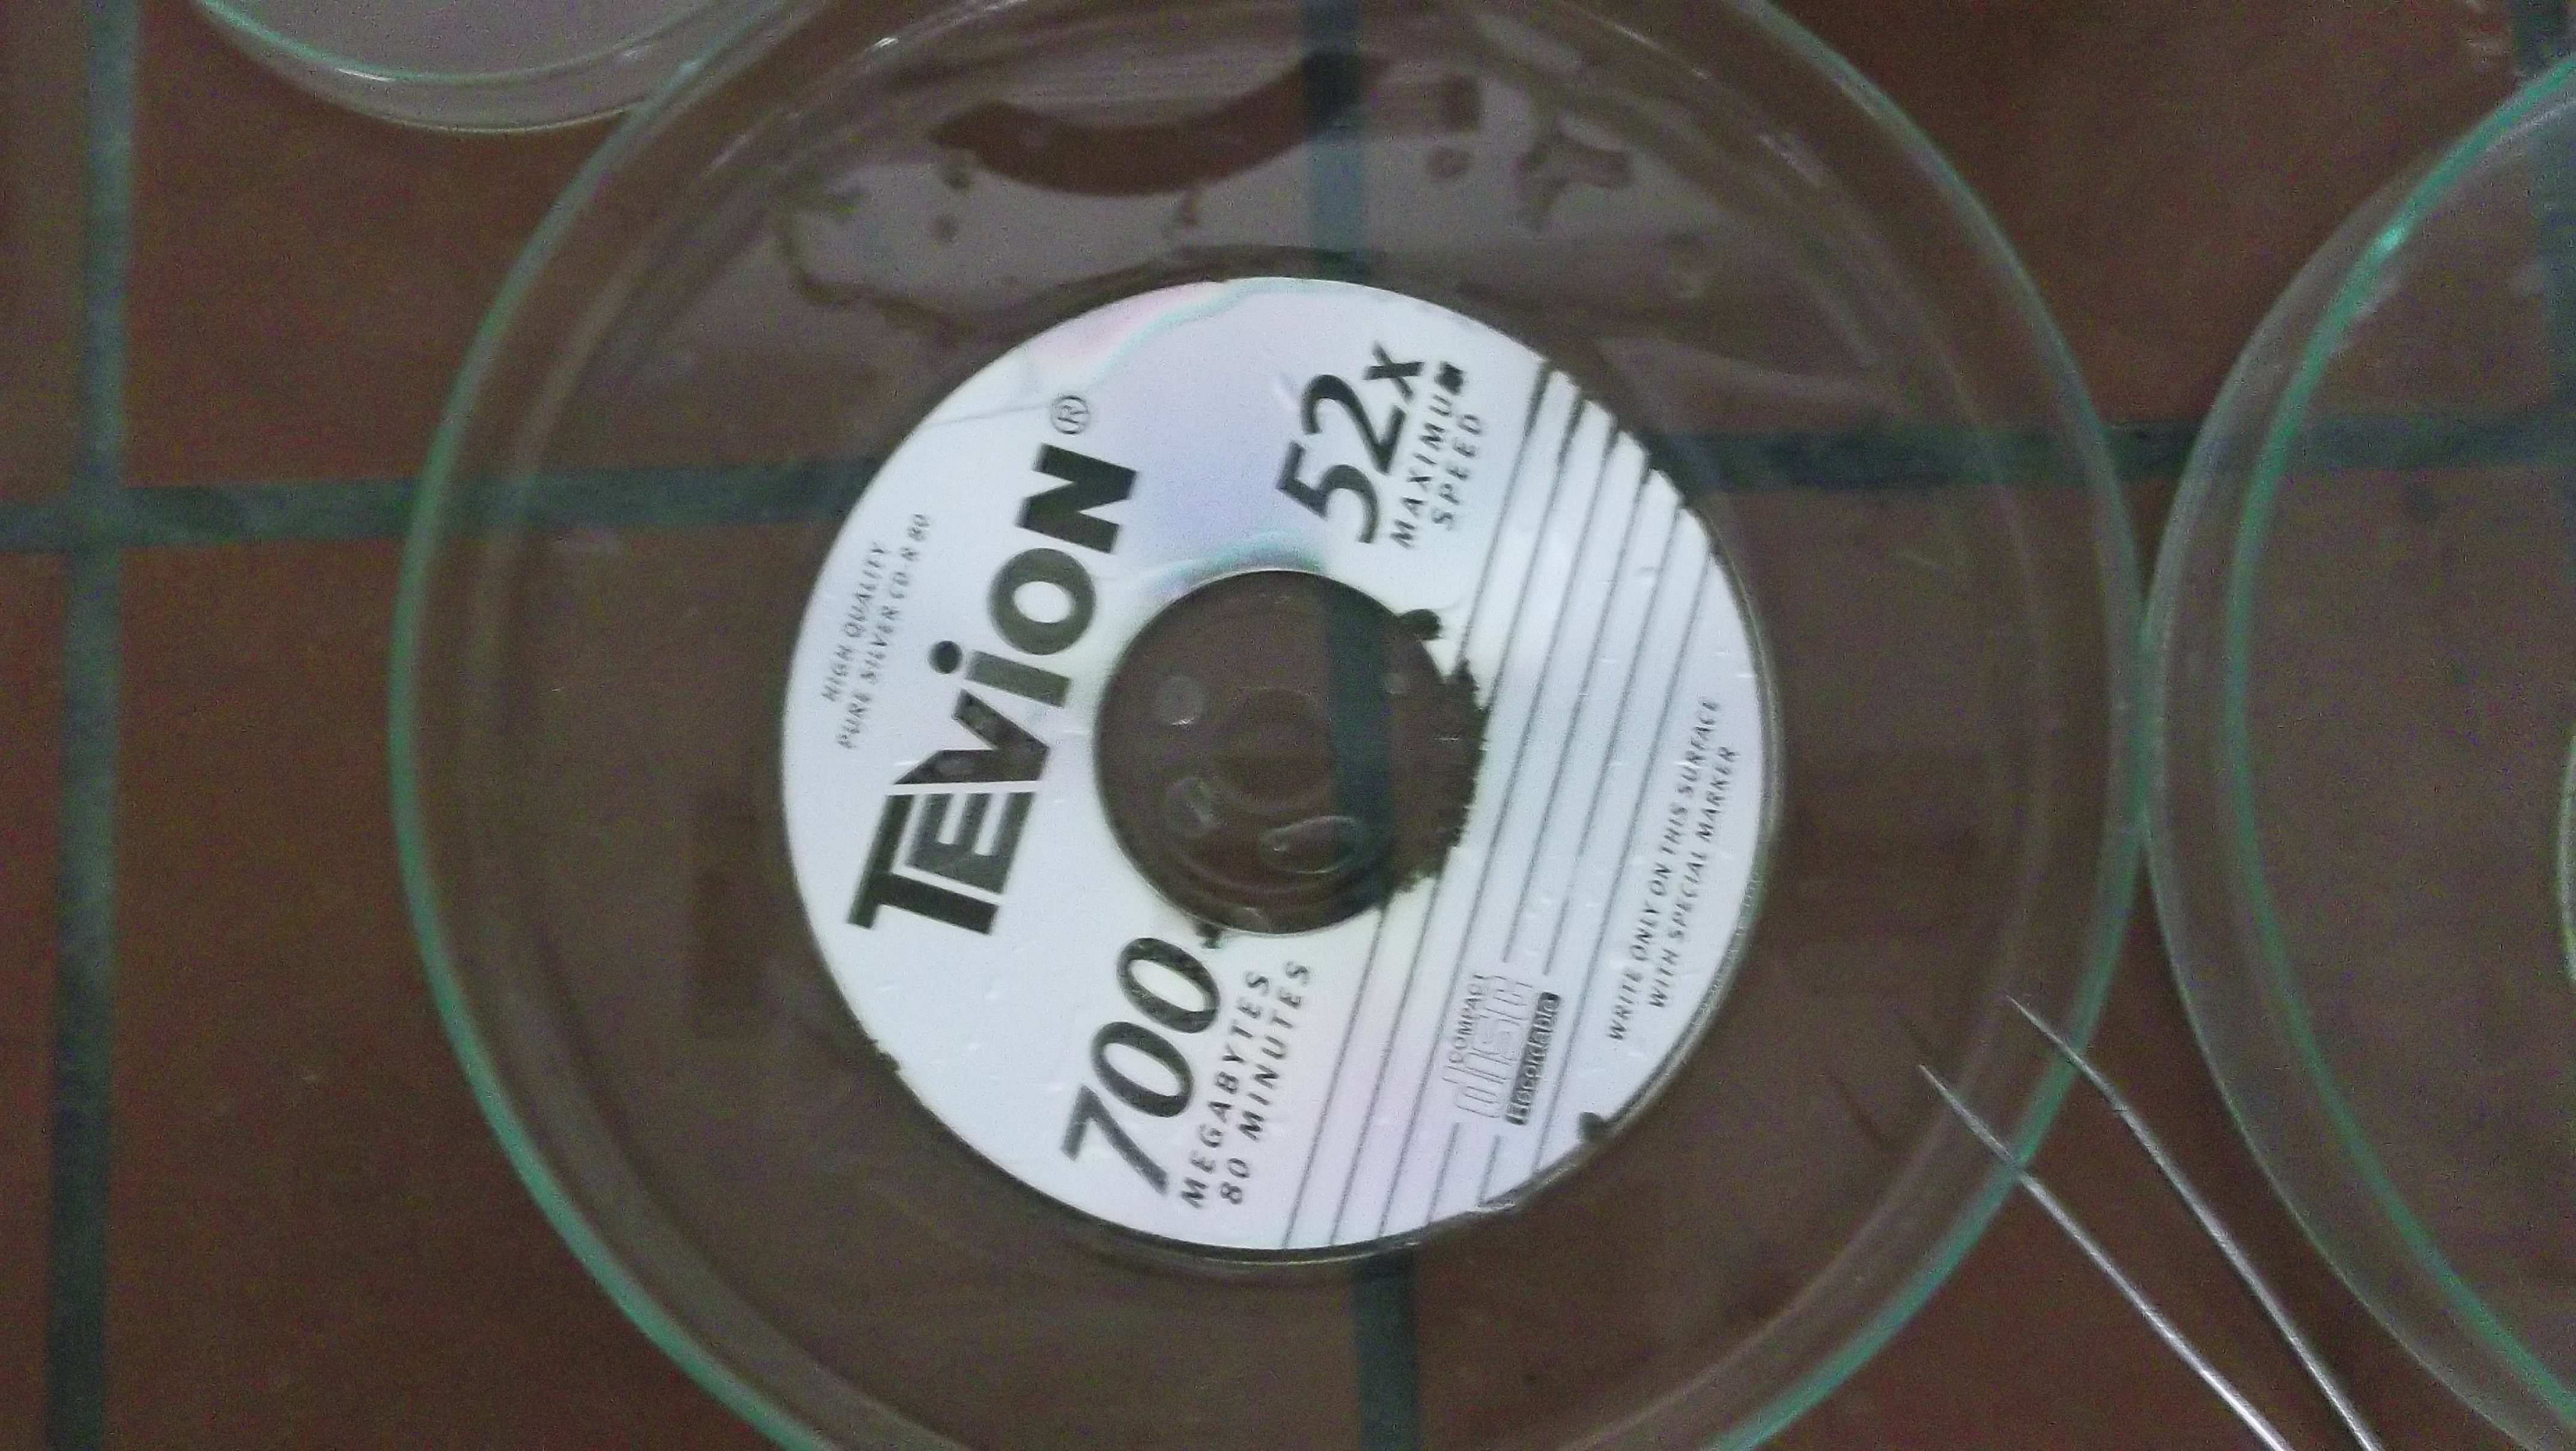
\includegraphics[height=0.1\textheight]{Bilder/Optische_Datentraeger_Die_Compact_Disc/Material_Polycarbonat/cdsalpeter.png}
                \caption[CD in Salpetersäure]{CD in Salpetersäure}
                \label{fig:cdsalpeter}
            \end{center}
        \end{minipage}
        \hspace{0.025\textwidth}
        \begin{minipage}[t]{0.4\textwidth}
            \begin{center}
                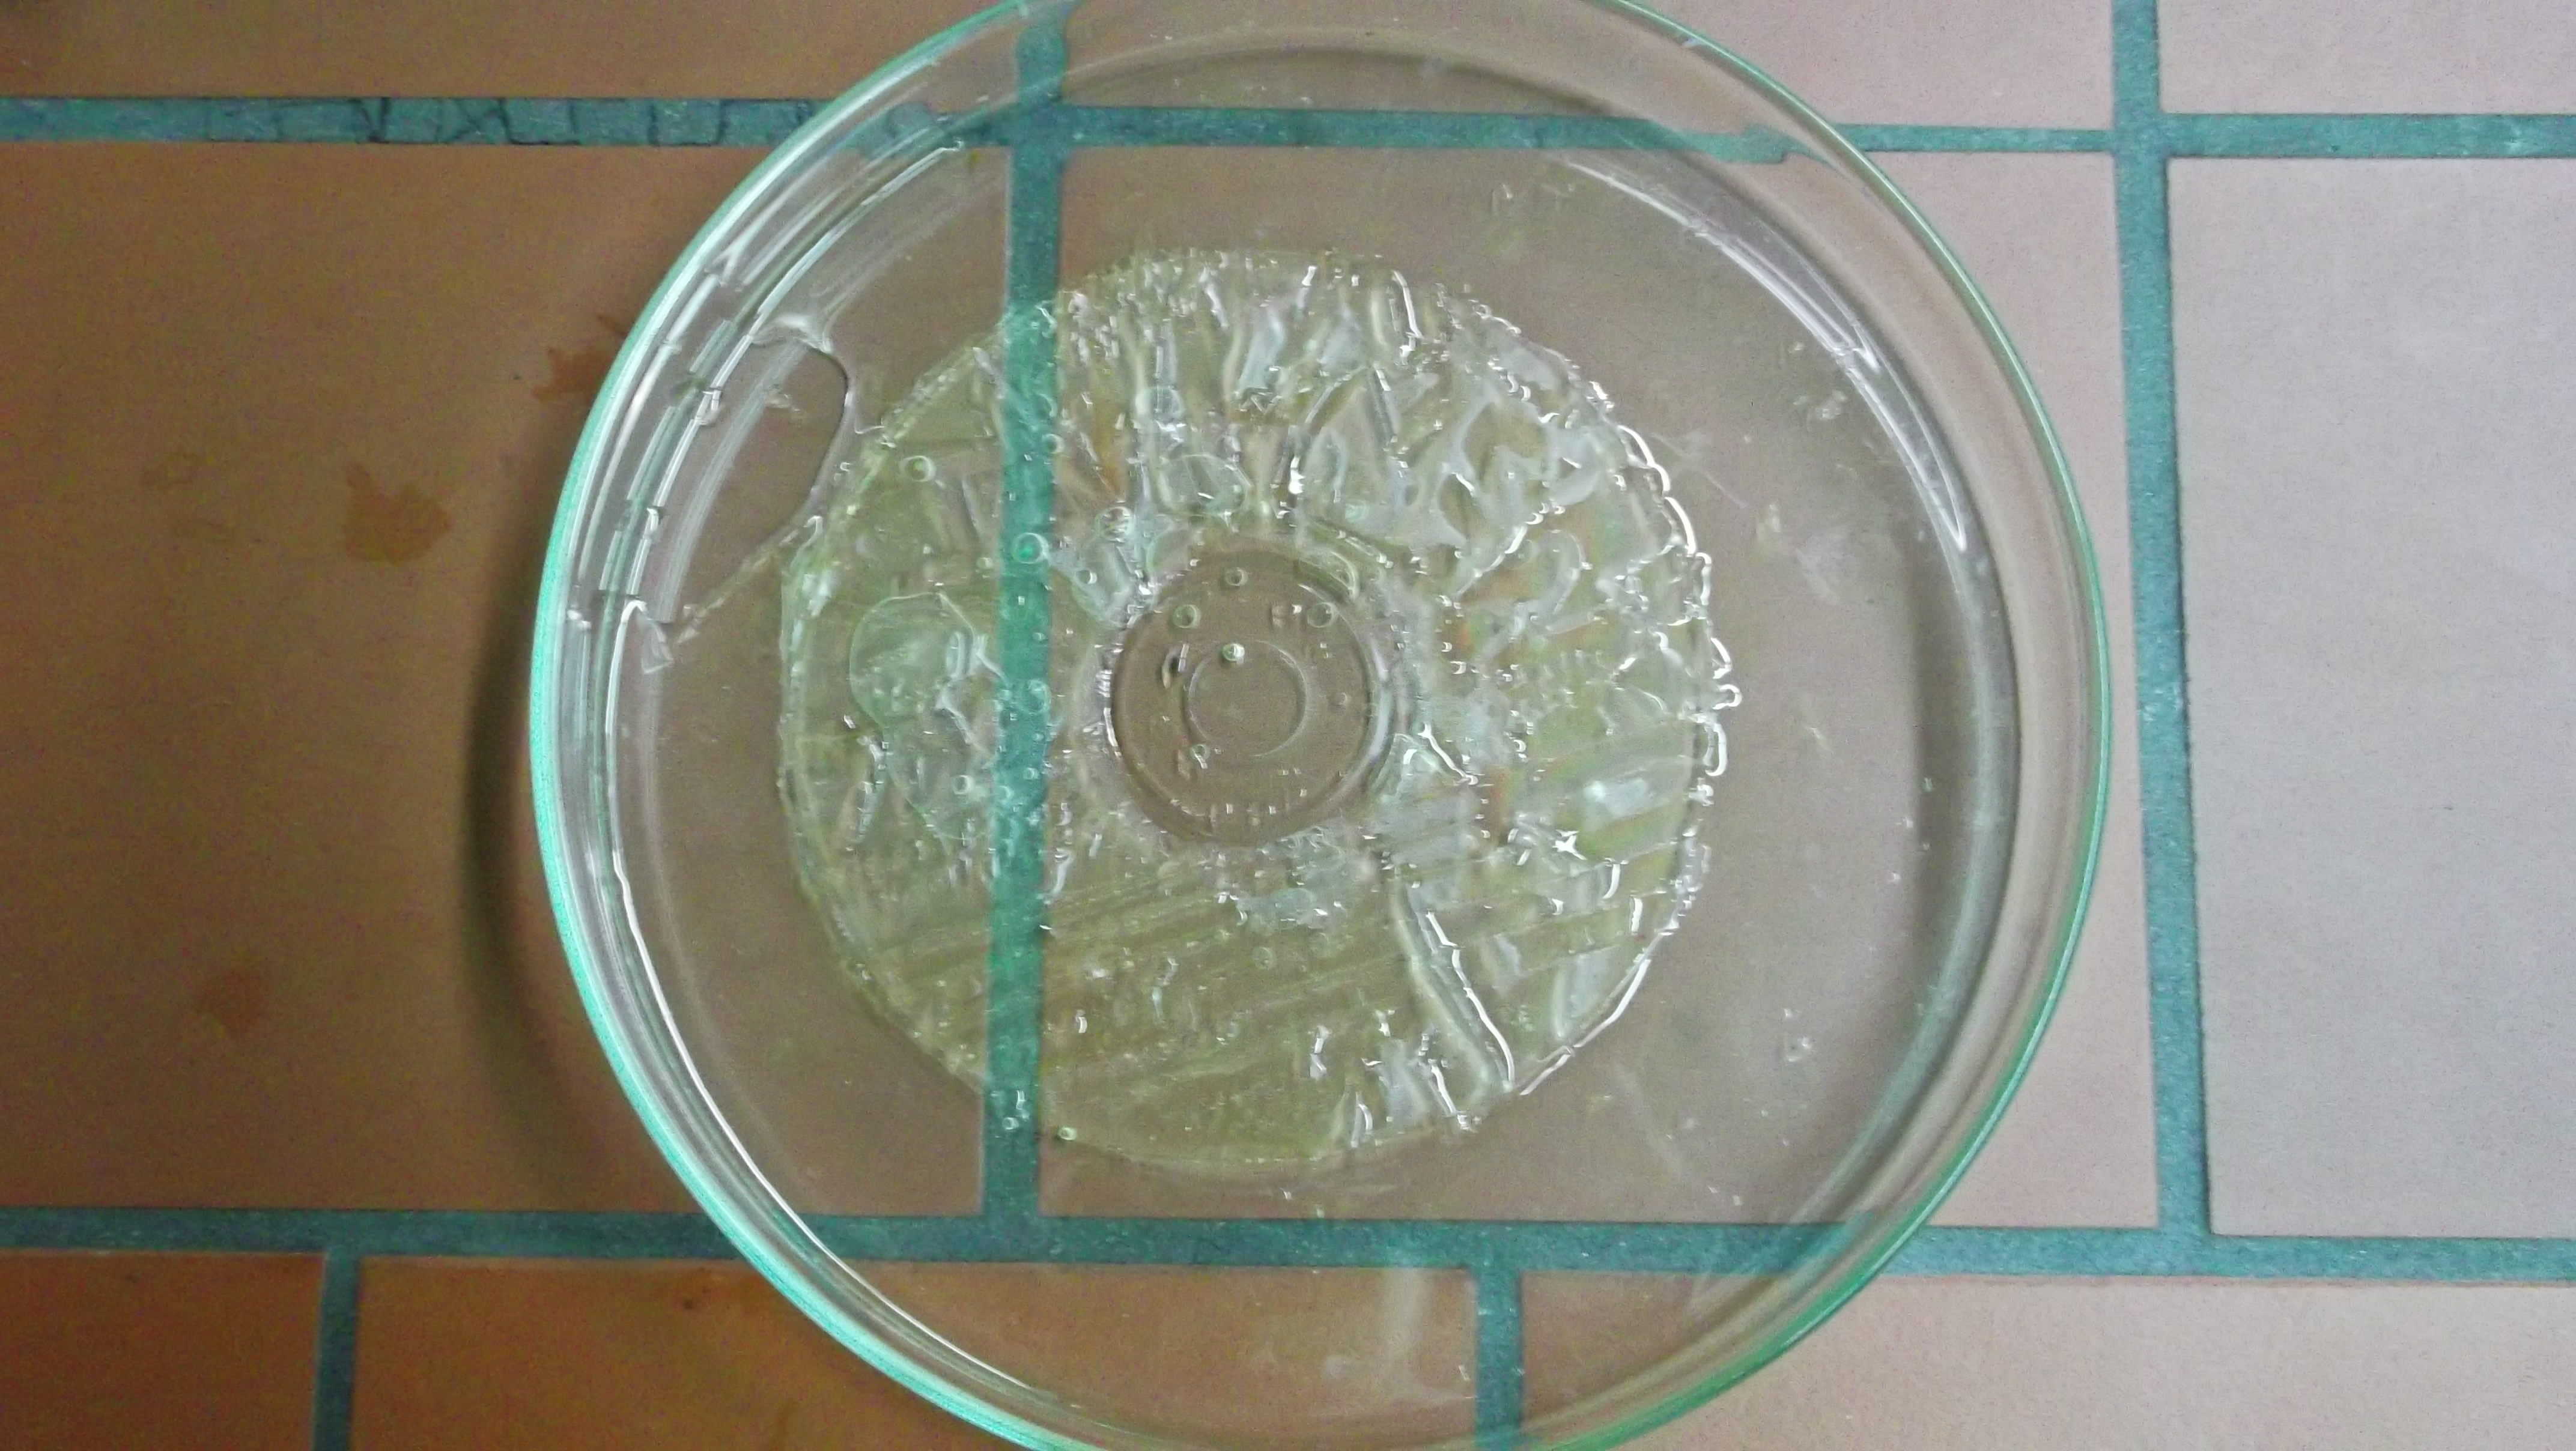
\includegraphics[height=0.1\textheight]{Bilder/Optische_Datentraeger_Die_Compact_Disc/Material_Polycarbonat/cdquillt.png}
                \caption[\qlqq Aufgequolleney\grqq{} Lack- und Aluminiumschicht]{\glqq Aufgequollene\grqq{} Lack- und Aluminiumschicht}
                \label{fig:cdquillt}
            \end{center}
        \end{minipage}
    \end{center}
\end{figure}

\begin{figure}[h]
    \begin{center}
        \begin{minipage}[t]{0.4\textwidth}
            \begin{center}
                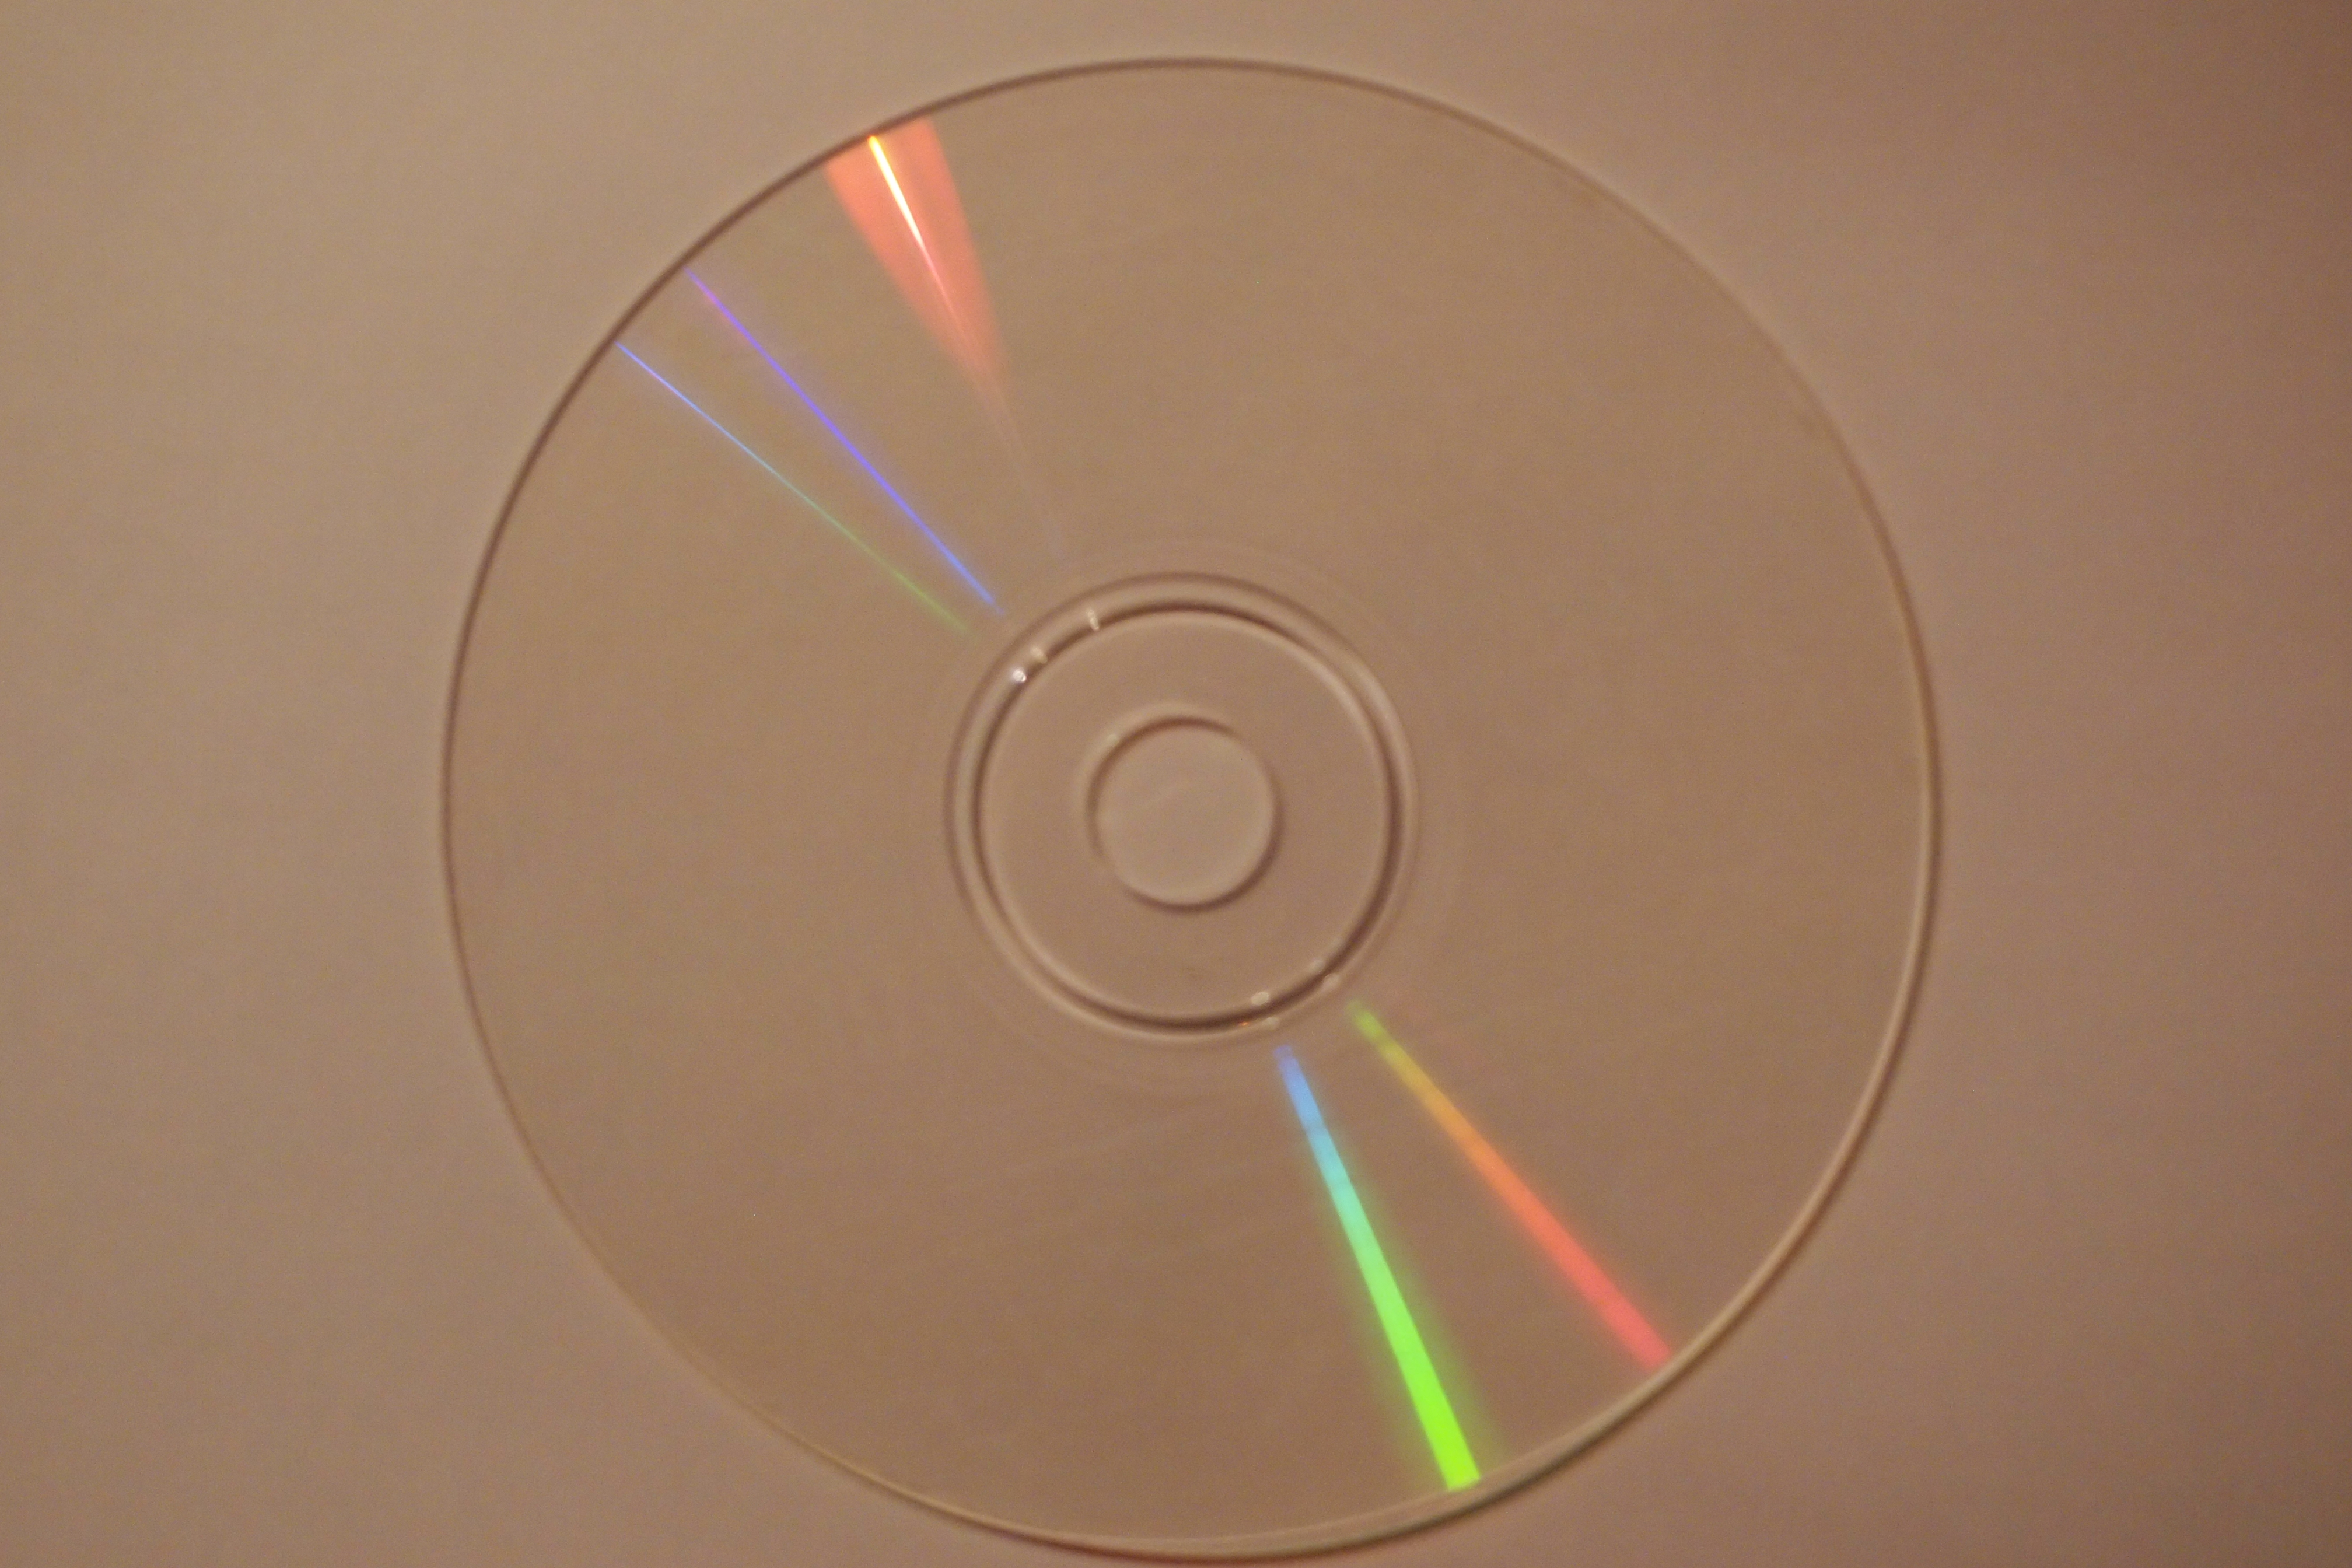
\includegraphics[height=0.1\textheight]{Bilder/Optische_Datentraeger_Die_Compact_Disc/Material_Polycarbonat/cdblank.png}
                \caption[Polycarbonatscheibe]{Polycarbonatscheibe}
                \label{fig:cdblank}
            \end{center}
        \end{minipage}
        \hspace{0.025\textwidth}
        \begin{minipage}[t]{0.4\textwidth}
            \begin{center}
                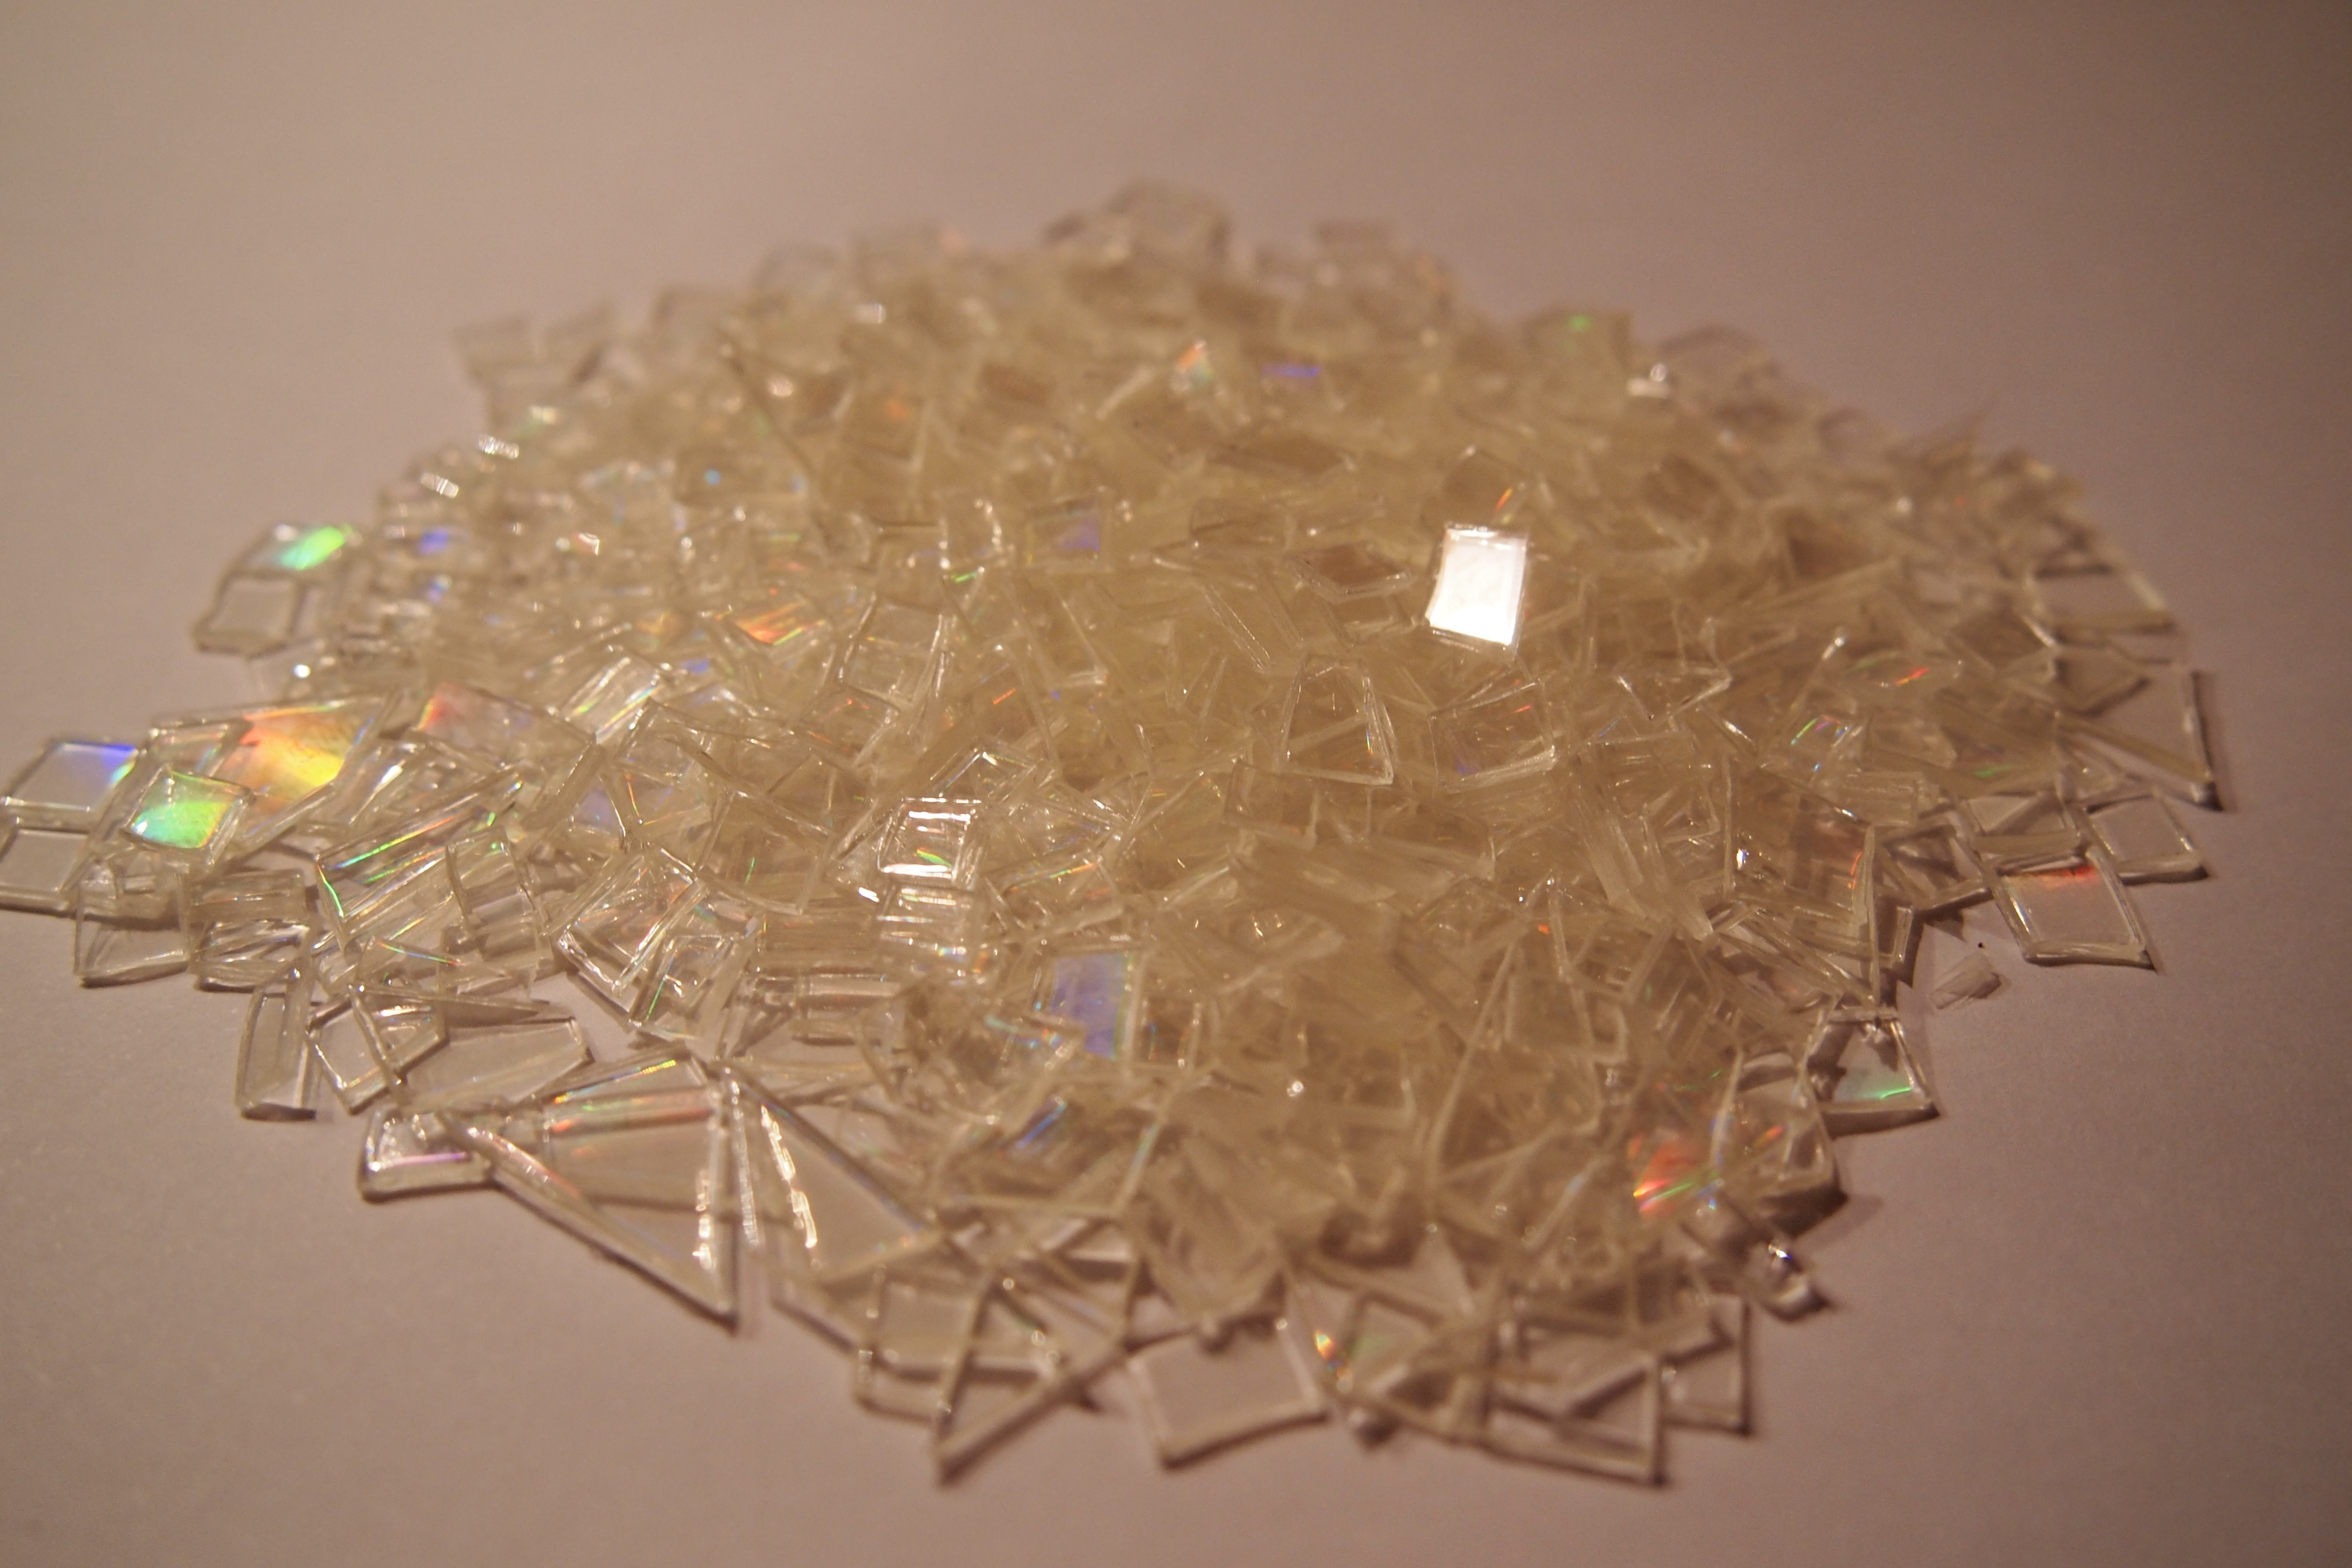
\includegraphics[height=0.1\textheight]{Bilder/Optische_Datentraeger_Die_Compact_Disc/Material_Polycarbonat/cdzerschnitten.png}
                \caption[CD in kleine Stücke zerschnitten]{CD in kleine Stücke zerschnitten}
                \label{fig:cdzerschnitten}
            \end{center}
        \end{minipage}
    \end{center}
\end{figure}

\begin{figure}[h]
    \begin{center}
        \begin{minipage}[t]{0.4\textwidth}
            \begin{center}
                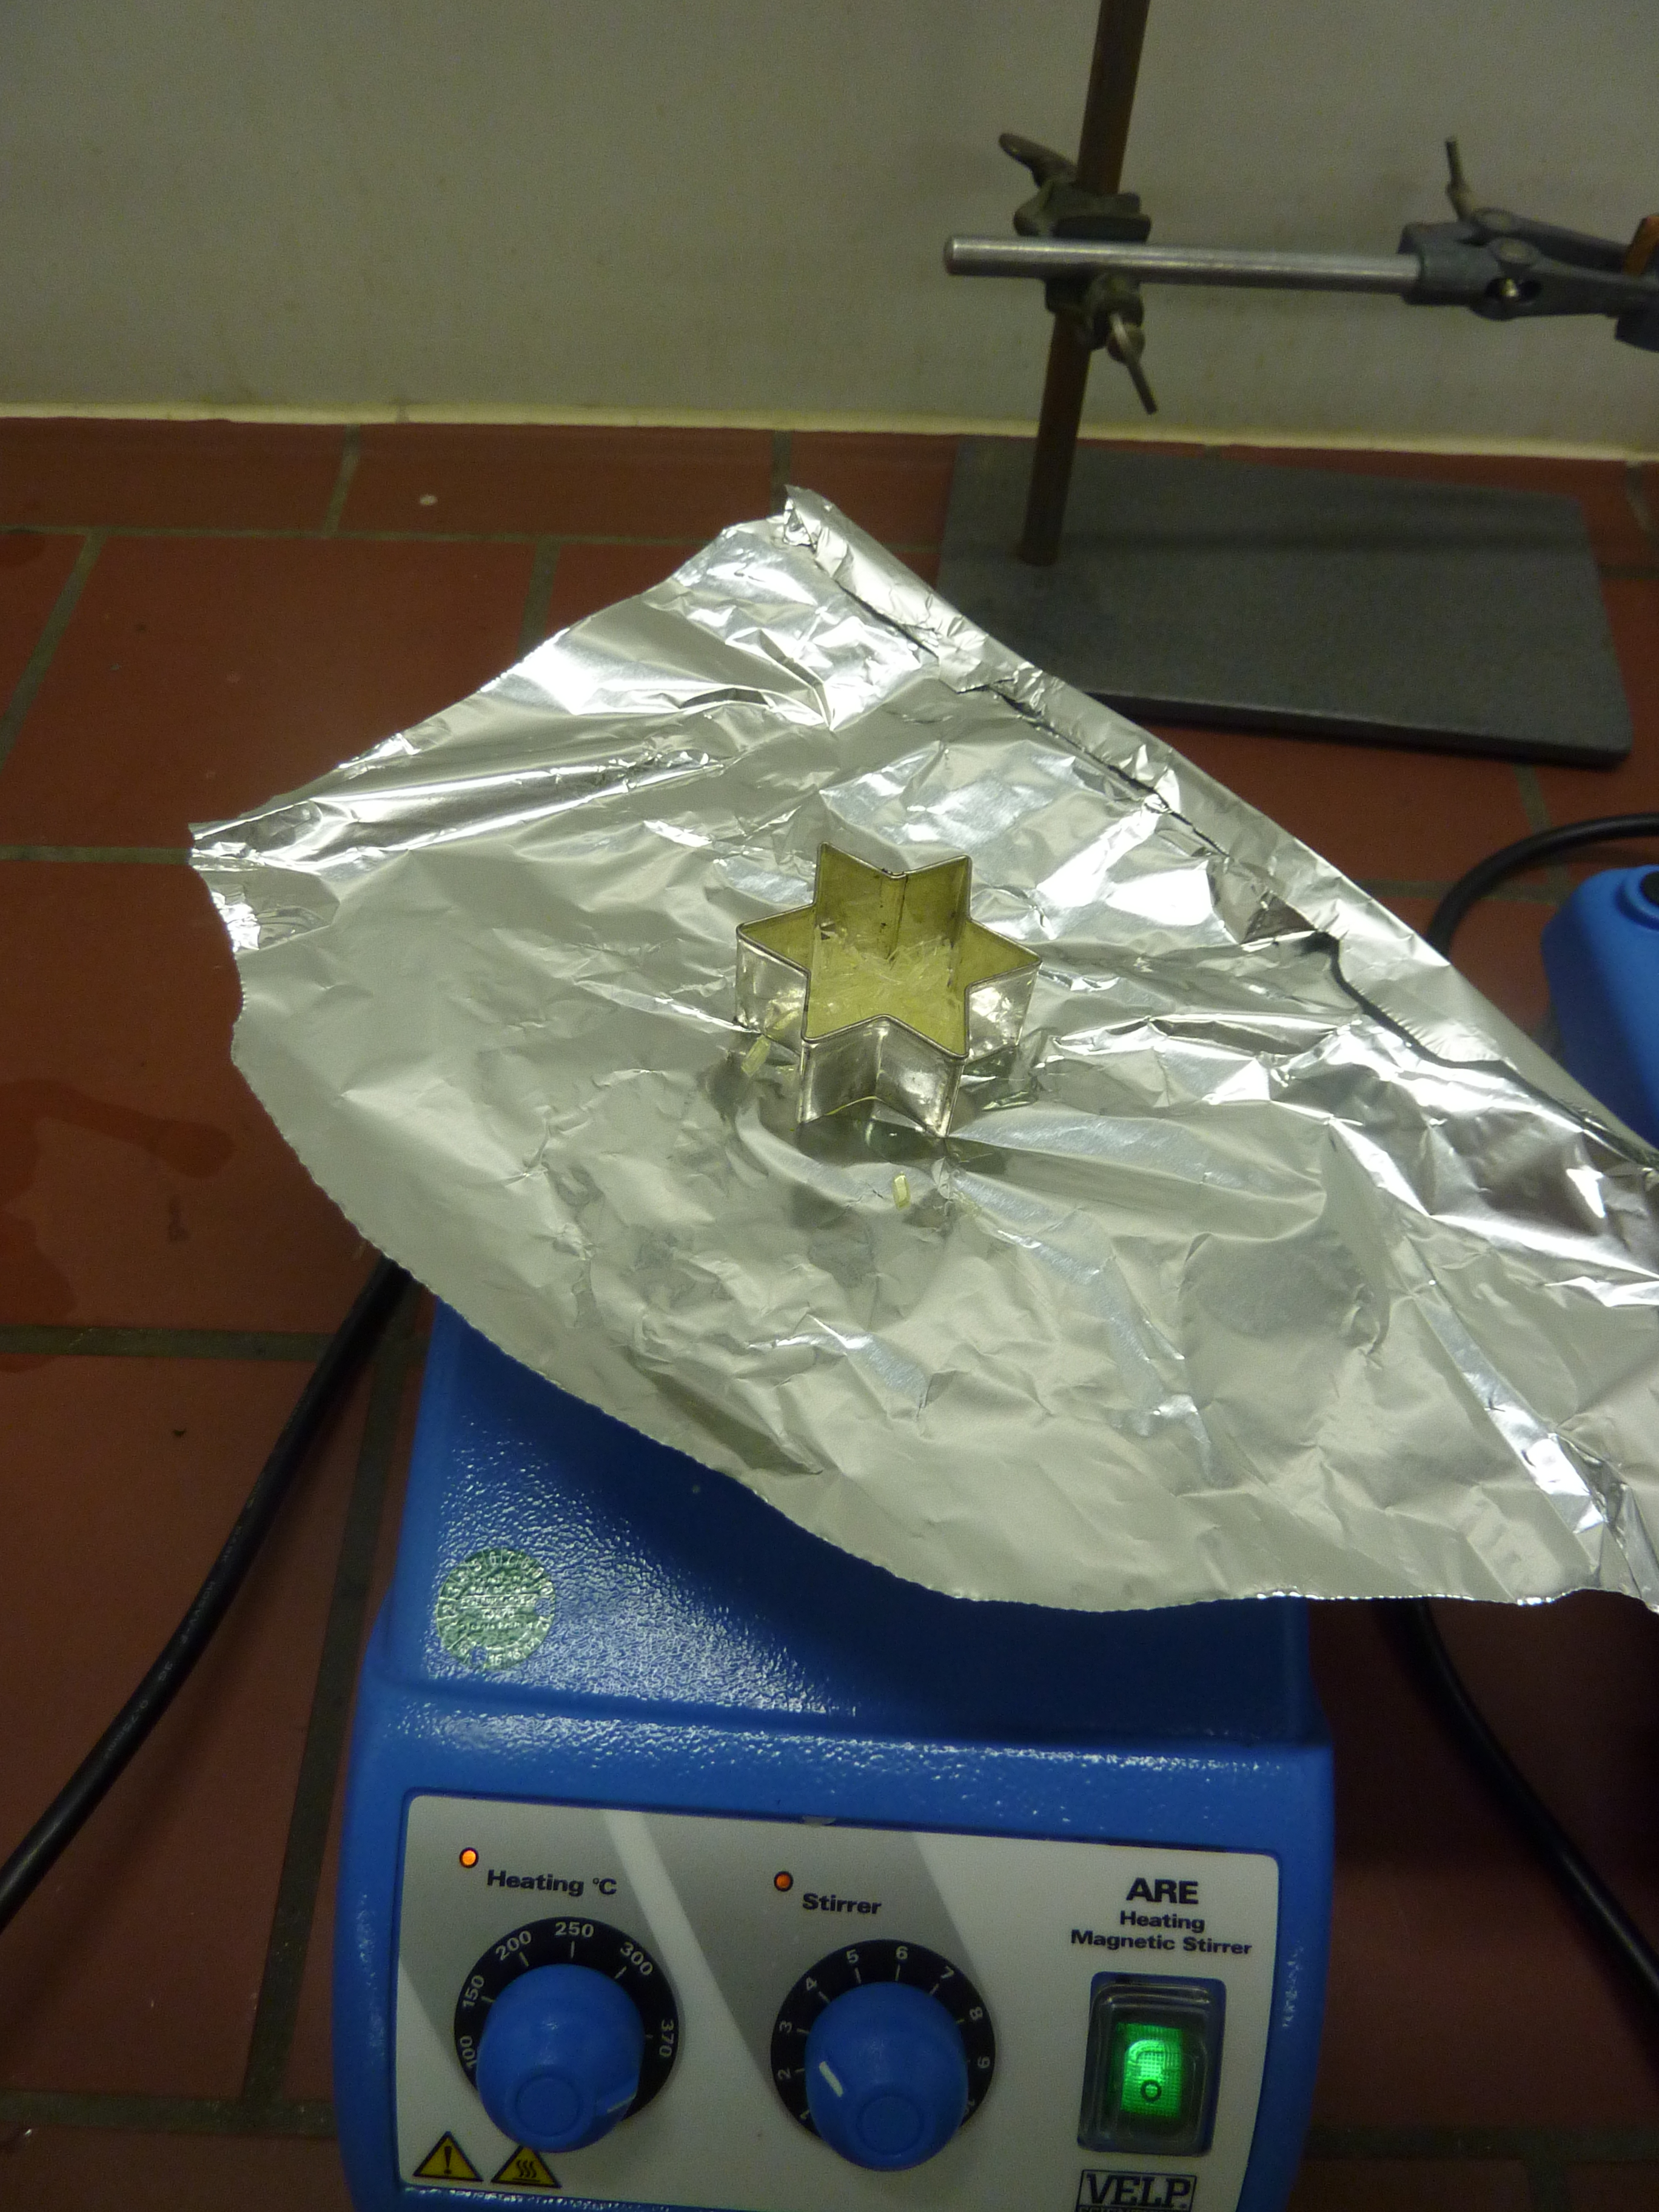
\includegraphics[height=0.1\textheight]{Bilder/Optische_Datentraeger_Die_Compact_Disc/Material_Polycarbonat/cdschmelzen.png}
                \caption[Heizplatte mit Plätzchenform]{Heizplatte mit Plätzchenform}
                \label{fig:cdschmelzen}
            \end{center}
        \end{minipage}
        \hspace{0.025\textwidth}
        \begin{minipage}[t]{0.4\textwidth}
            \begin{center}
                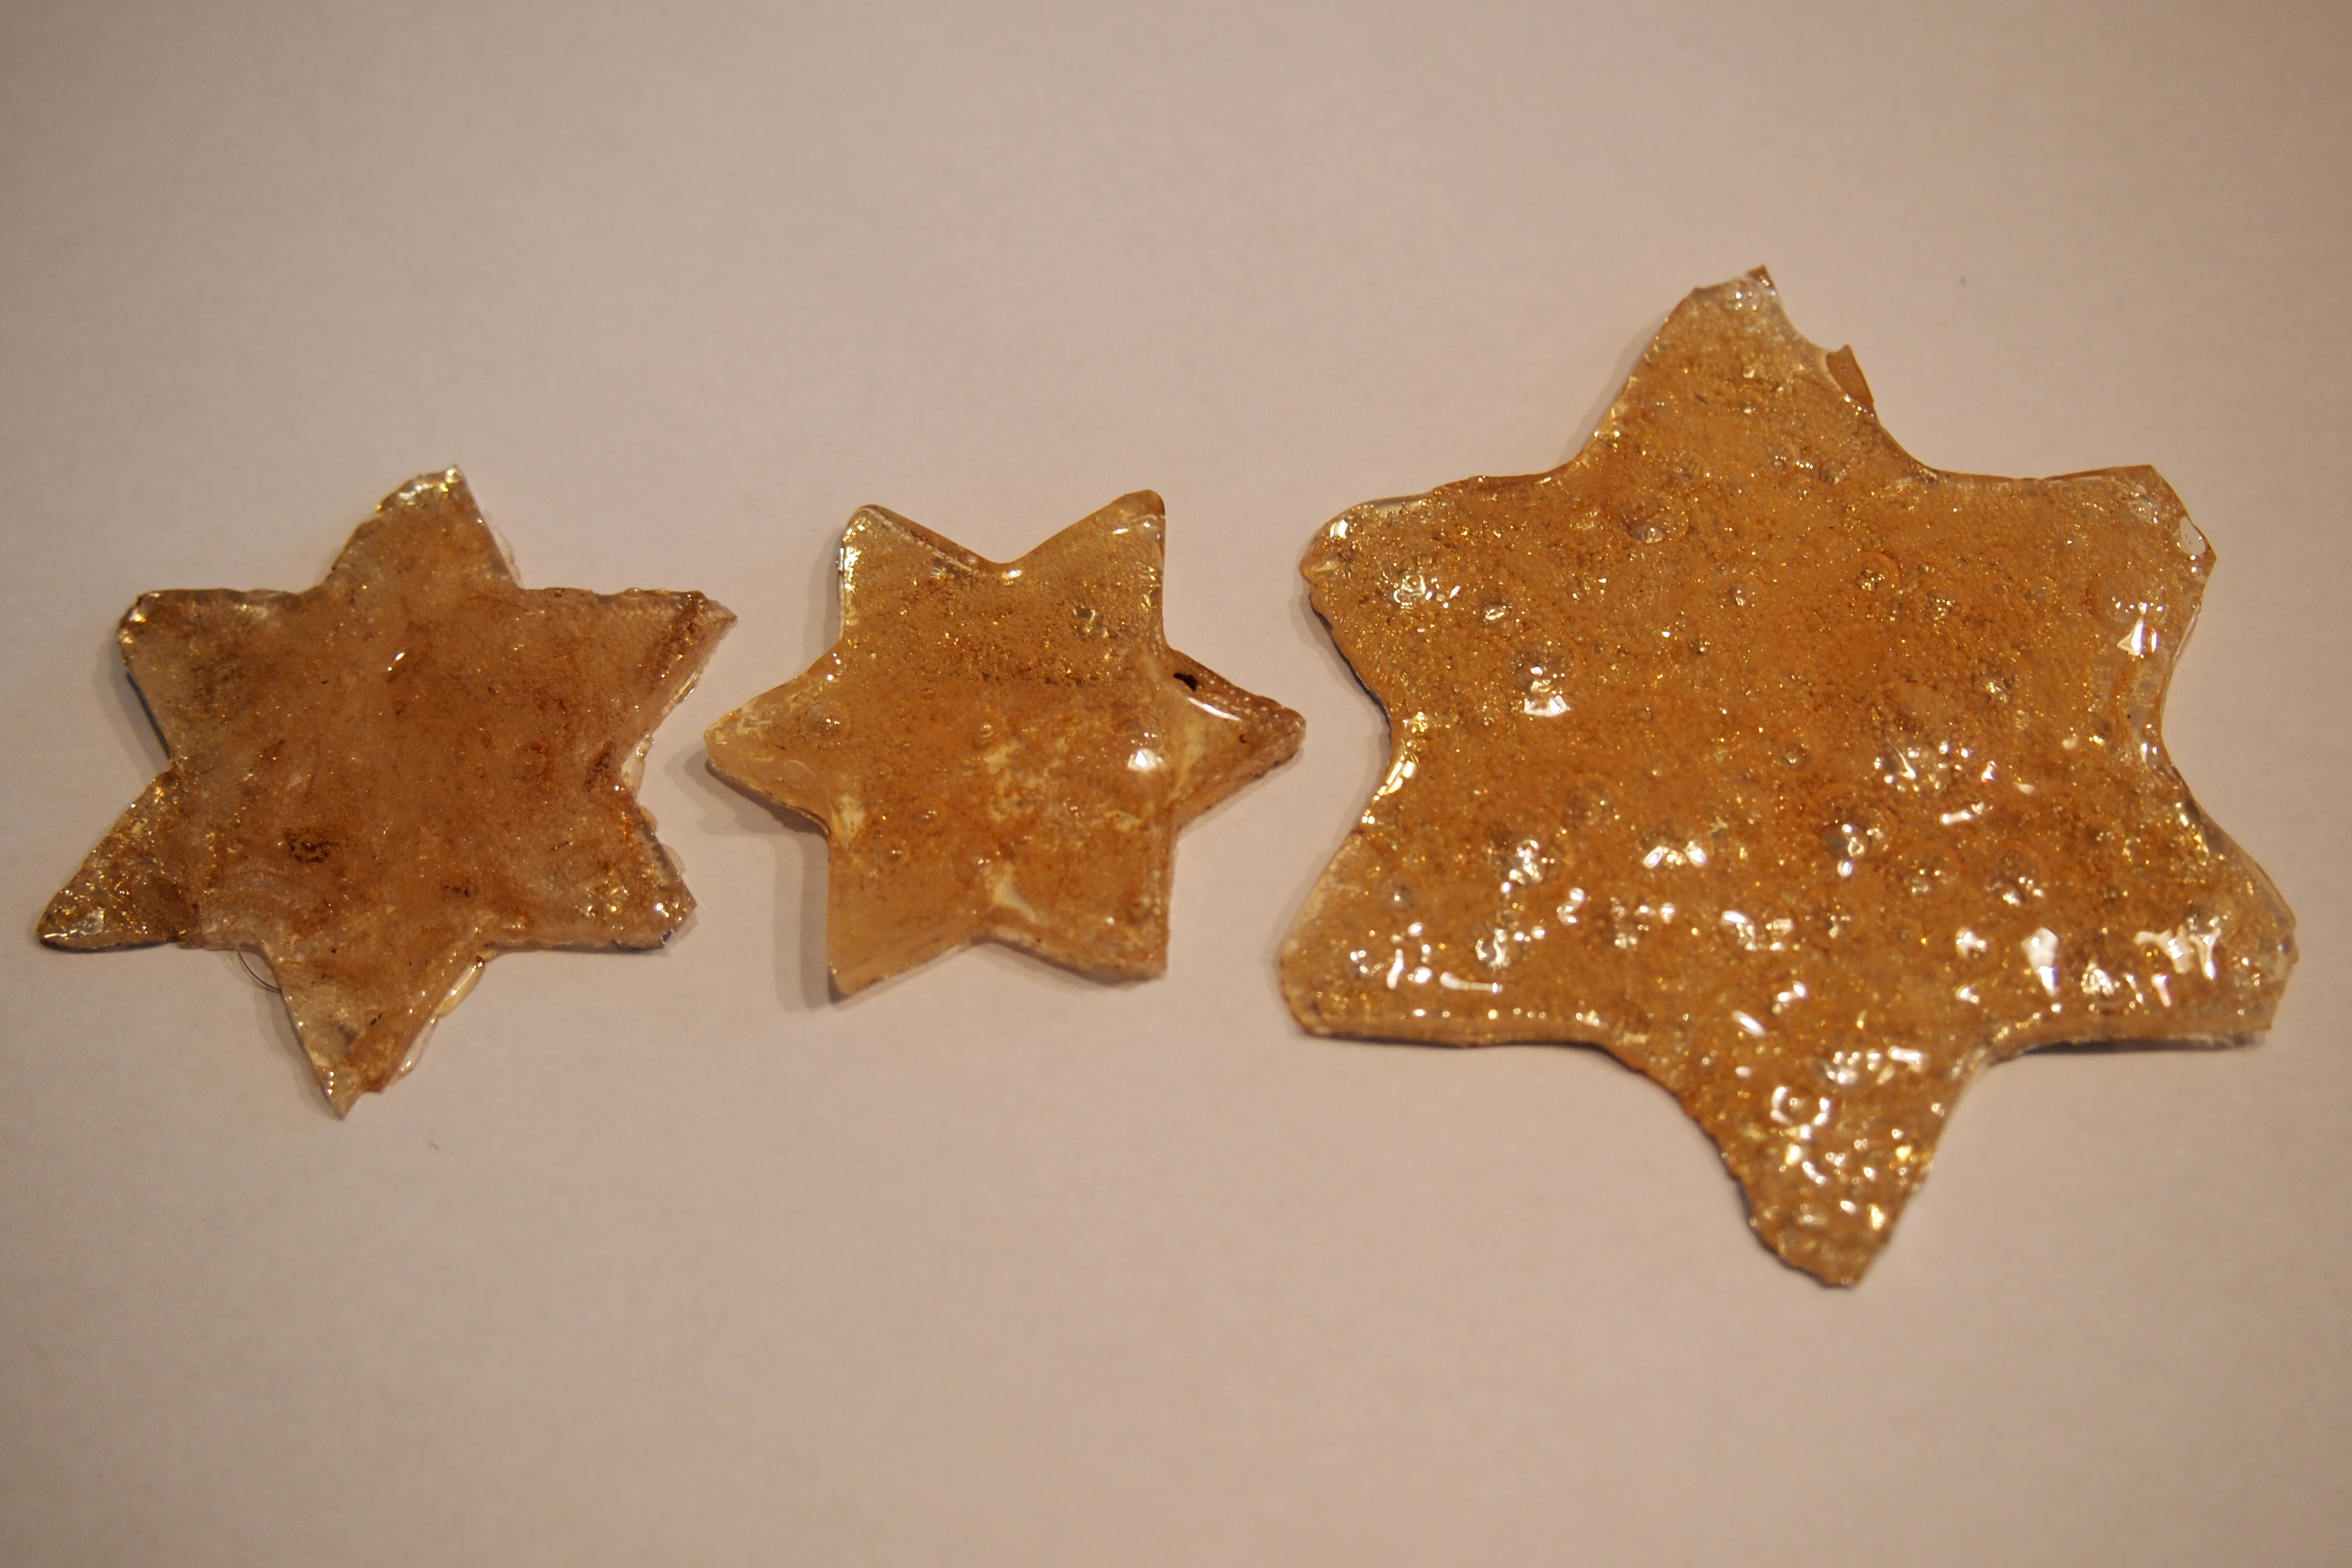
\includegraphics[height=0.1\textheight]{Bilder/Optische_Datentraeger_Die_Compact_Disc/Material_Polycarbonat/cdplaetzchen.png}
                \caption[\glqq Polycarbonatplätzchen\grqq{}]{\glqq Polycarbonatplätzchen\grqq{}}
                \label{fig:cdplaetzchen}
            \end{center}
        \end{minipage}
    \end{center}
\end{figure}

Ergebnisse des Versuchs:
\begin{enumerate*}
    \item hohe Lichtdurchlässigkeit: Wird die \shorthandoff{"}"gehäutete"\shorthandon{"} Polycarbonatscheibe in das CD-Laufwerk eines Computers eingelegt, erkennt dieser nicht, dass eine CD eingelegt wurde, da der Laserstrahl ungehindert durch die Polycarbonatscheibe geht. Dies beweist ebenfalls, dass die Aluminiumschicht für die Reflektion des Laserstrahls verantwortlich ist.
    \item einfache Weiterverarbeitung: Die Polycarbonatschnipsel lassen sich ohne großen Aufwand und innerhalb kurzer Zeit in eine neue Form schmelzen. Die Qualitätsminderung liegt an den Verschmutzungen, die aufgrund der primitiven Methode zum Einschmelzen unvermeiden ist.
\end{enumerate*}
